\documentclass[11pt]{article}

\usepackage{metaagent-paper}

\graphicspath{{figures/}{docs/paper/latex/figures/}}

\title{\vspace{-1.2em}Towards automated screening and coding for infectious disease systematic reviews with large language models}

\author[1]{Author}
\affil[1]{Affiliation 1, Department, Institution, City, Country}


\date{Updated @ \DTMtoday}

\begin{document}
\maketitle

\begin{abstract}
Systematic reviews underpin parameterization of infectious disease models but are limited by labor-intensive screening of large literature corpora with low inclusion yield. Although large language models (LLMs) show promise for automation, their performance in literature screening remains suboptimal without domain-specific design. Here, we present a dimension-aware LLM framework for literature screening, evaluating articles across three epidemiological characteristics: transmission potential, transmission speed, and disease severity. Using a benchmark of 22 COVID-19 and mpox systematic review profiles (12,758 records; 668 included studies), the model achieves consistently high recall across parameters: 0.984 (95\% CI: 0.959--0.994) for reproduction number, 0.935 (95\% CI: 0.894--0.961) for serial interval, and 0.957 (95\% CI: 0.919--0.977) for fatality; and reduces manual screening workload by 60\% (95\% CI: 0.59--0.62), 83\% (95\% CI: 0.82--0.84), and 76\% (95\% CI: 0.75--0.77), respectively. These findings demonstrate that dimension-aware LLMs can substantially improve screening efficiency while preserving high sensitivity, supporting their role as assistive tools in human-in-the-loop systematic review workflows.
\end{abstract}

\section{Introduction}

Accurate epidemiological characteristics are essential for evidence-based public health decision-making during infectious disease outbreaks.\cite{ref1,ref2,ref3,ref4} Parameters such as the basic reproduction number ($R_0$), serial interval, and case fatality rate serve as quantitative indicators of transmission potential, transmission speed, and disease severity, respectively. These parameters critically inform the development of public health strategies, the design of intervention measures, and the allocation of healthcare resources. However, obtaining reliable estimates of these parameters requires rigorous evidence synthesis.

Although parameter estimates from single high-impact studies or preliminary reports are commonly used, they often introduce substantial uncertainty and propagate systematic bias throughout model simulations, ultimately undermining the reliability and interpretability of projections. Systematic reviews and meta-analyses offer a superior alternative as the most authoritative source of such parameters. Through standardized integration of evidence across studies, they effectively reduce biases related to publication, geography, and population heterogeneity.\cite{ref5,ref6,ref7} Only by adopting parameters derived from such comprehensive evidence synthesis can transmission models move beyond theoretical constructs to deliver credible, policy-relevant predictions.

Nevertheless, despite generating high-quality evidence, the systematic review entails substantial resource requirements and considerable operational complexity. An empirical investigation of PROSPERO-registered projects has demonstrated that the average duration from protocol initiation to full publication of a systematic review extends to 67.3 weeks, about 1.29 years.\cite{ref8} Moreover, the literature screening process is particularly labor-intensive: initial database searches frequently retrieve tens of thousands of records, ranging from 27 to over 90,000, of which only about 2.94\% typically meet the prespecified eligibility criteria.\cite{ref8} Consequently, researchers must devote considerable effort to screening vast numbers of citations to identify a small set of eligible studies.

In response to this labor-intensive bottleneck, artificial intelligence has emerged as a promising solution. Recent advances in artificial intelligence (AI) have enabled AI-assisted tools to alleviate the burden of manual screening, with active learning algorithms demonstrating particular promise in prioritizing relevant citations while maintaining high sensitivity.\cite{ref9,ref10,ref11} Nevertheless, existing unmodified large language models remain incapable of independently executing the critical task of identifying and selecting relevant literature for systematic reviews. This limitation is starkly illustrated by the performance of three fully automated GPT-4-based approaches: Consensus GPT, Scholar GPT, and the native GPT web-browsing mode correctly identified merely 32.7\% (32/98), 19.4\% (19/98), and 6.1\% (6/98) of eligible articles, respectively.\cite{ref12} These poor results highlight the need for domain-specific adaptation. While specialized models such as MedCPT in biomedical information retrieval\cite{ref13} and TrialMind in clinical trial screening\cite{ref14} have shown substantially better performance, the field of AI-assisted systematic review still lacks a dedicated, high-performance retrieval framework.

Here, we present \metagent{}, a dimension-aware large language model framework developed for high-recall literature screening in systematic reviews of infectious disease modeling parameters. The framework evaluates each candidate article across five clinically and methodologically relevant dimensions: disease relevance, population relevance, location relevance, original empirical evidence, and parameter relevance; and employs a stage-aware screening strategy that adapts the input modality according to the availability of title and abstract information. By integrating these design elements, \metagent{} aims to preserve high sensitivity while substantially reducing the manual screening burden. This study demonstrates that dimension-aware LLMs can serve as effective assistive tools within human-in-the-loop systematic review workflows, providing a practical pathway to accelerate high-quality evidence synthesis for infectious disease modeling and public health decision-making.

% !TEX root = ../main.tex
\section{Method}

We developed a framework named \metagent{} for automated literature screening and full-text parameter coding in systematic reviews of infectious disease modeling (Figure~\ref{fig:pipeline}). The proposed \metagent{} comprises three core components: benchmark construction, LLM screening, and full-text parameter coding and extraction. Performance was evaluated separately for the screening and coding components: the screening output was evaluated against the review-derived inclusion lists, while the coding output was evaluated against the estimates reported by the source reviews.

\begin{figure}[!t]
  \centering
  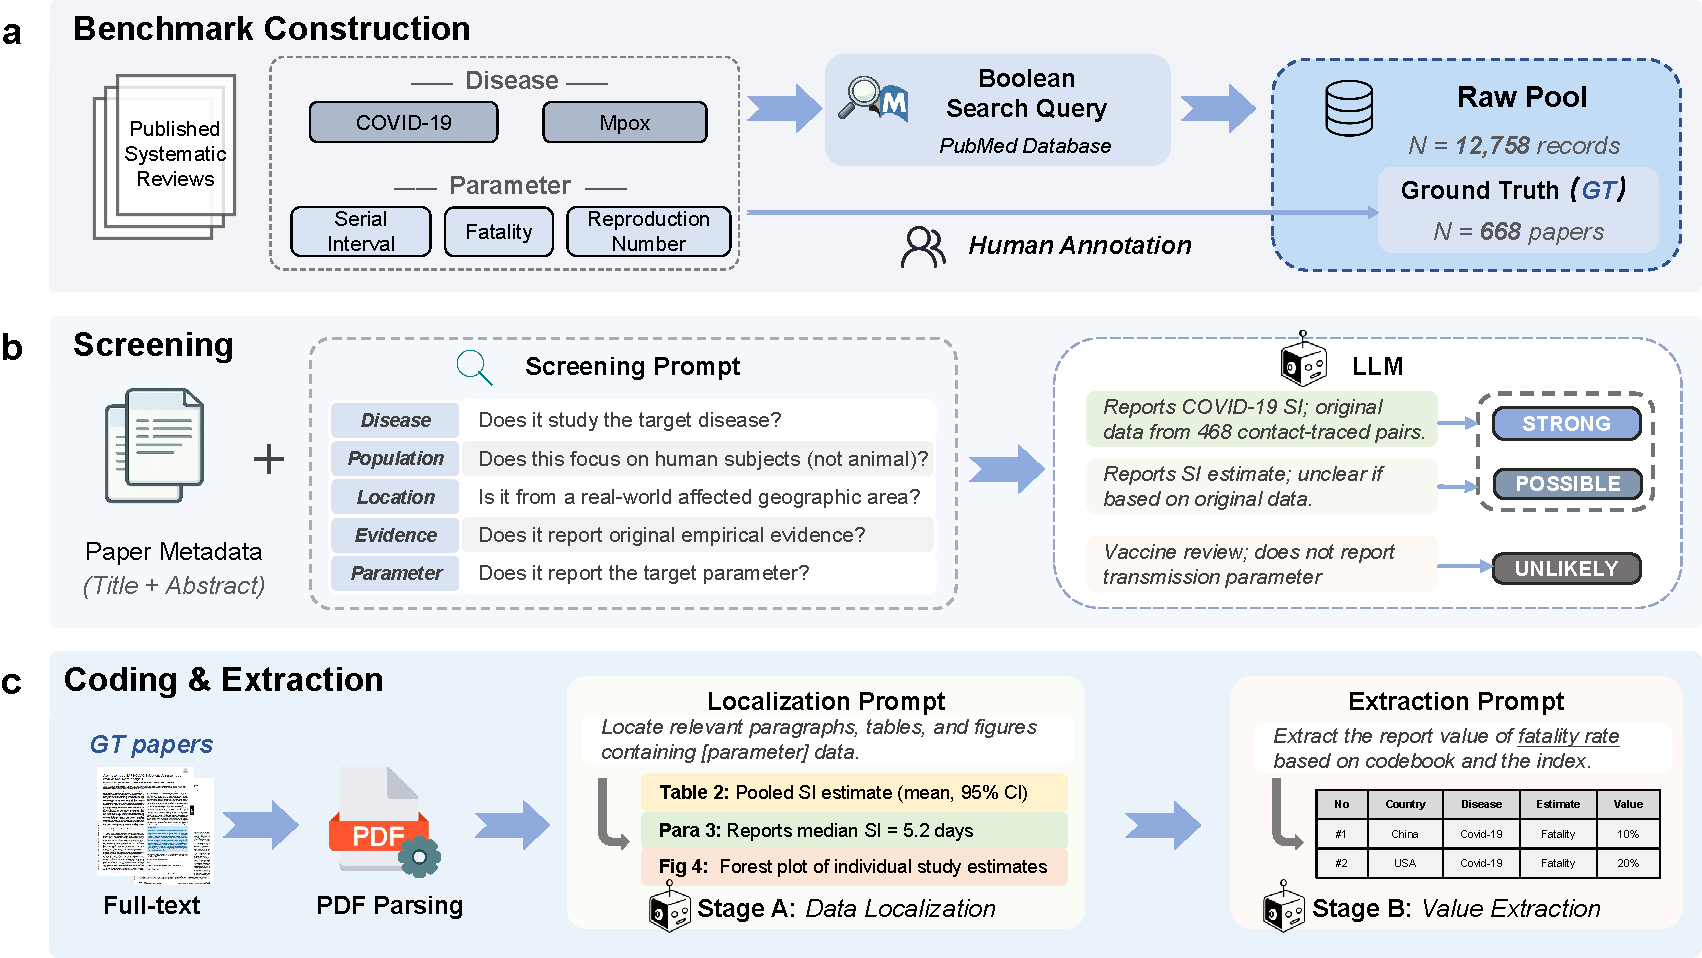
\includegraphics[width=\textwidth]{pipeline/pipeline.pdf}
  \caption{Overview of the \metagent{} pipeline. a) Benchmark construction from published systematic reviews, defining the raw pool of candidate records and the review-derived ground truth. b) LLM-assisted screening based on title-and-abstract metadata, in which a five-criterion screening prompt (disease, population, location, empirical evidence, target parameter) maps each record to Strong, Possible, or Unlikely. c) Full-text parameter coding and extraction comprising data localization (Stage A) and codebook-guided value extraction (Stage B) over the source-review included studies. Evaluation was performed separately for screening and coding outputs and is not shown as a pipeline panel.}
  \label{fig:pipeline}
\end{figure}

\subsection{Benchmark Construction}

This study selected three core epidemiological parameters to evaluate the proposed screening framework: basic reproduction number ($R_0$), serial interval, and fatality, characterizing the transmission potential, transmission speed, and disease severity of an epidemic. We constructed a screening benchmark from published systematic reviews on COVID-19/SARS-CoV-2 and mpox. The benchmark comprises 22 source-review screening tasks, each corresponding to one published systematic review, with a total of 12,758 candidate records. The source reviews used to define the benchmark are listed in Table~\ref{tab:source-reviews}. For each task, we designed a Boolean search query based on the target parameter definitions, using the same search time frame and adhering as closely as possible to the original search strategies reported in the source reviews. PubMed served as the primary data source for retrieving records, which collectively formed the raw pool of candidate articles for screening.

Upon constructing the raw pool, we defined the final inclusion list of each systematic review as the corresponding ground truth (GT) for that task. In this framework, the raw pool delineates the search space of candidate records, whereas the GT identifies the subset of articles that should ultimately be included. Across the benchmark, the aggregated GT consists of 668 articles. It is important to emphasize that the GT in this study does not constitute a rigorous gold standard in the strictest sense. The original search strategies often relied on multiple bibliographic databases and could not be fully reconstructed from the published manuscripts alone, meaning that some GT articles may not appear in our constructed raw pool. The original reviews may themselves contain retrieval omissions or include eligibility constraints that are not fully encoded in the current tasks.

For the coding evaluation, each source review additionally contributed one manually abstracted reference estimate from the source-review report. When available, we selected the reported overall or primary pooled estimate for the target parameter, together with its 95\% confidence interval or reported uncertainty interval. When a source review reported multiple subgroup-, setting-, variant-, or period-specific estimates and did not provide a single overall value, the selected target followed the review's stated primary synthesis question and the included-study evidence available for coding, rather than forcing all reviews into a common estimand. This procedure fixed a transparent review-derived benchmark target for each source review; it was not intended to independently adjudicate whether the source review's own estimate was error-free. The selected reference estimates and uncertainty intervals used in each comparison are listed in Appendix D, enabling readers to audit the target used for each source-review comparison.

\subsection{LLM Screening}

\textbf{Task definition.}
We formulate the task as high-recall first-pass screening, rather than a definitive inclusion/exclusion decision. The objective of the system is to maximally retain GT-positive articles while substantially reducing the number of records requiring manual review, thereby focusing human effort on studies with a higher likelihood of relevance. Final inclusion judgments remain the responsibility of domain experts operating at the full-text level.

\textbf{Screening input.}
Each candidate record was screened on the basis of its bibliographic metadata, comprising the title and the abstract retrieved from PubMed (Figure~\ref{fig:pipeline}b). The same screening prompt and the same Strong, Possible, or Unlikely triage rule were applied uniformly to all records, without auxiliary retrieval or full-text access. When an abstract was unavailable, as occurs for certain preprint records, letters, or older publications with incomplete metadata, the input was reduced to the title alone, while the eligibility criteria remained unchanged; records that could not be confidently excluded from the title alone were retained for downstream review.
% This unified input formulation reflects the operating conditions of a typical database-driven first-pass screening task and isolates the reported screening performance from variability introduced by full-text retrieval or document parsing.

\textbf{Screening prompt.}
Given the title-and-abstract input defined above, the screening prompt structures the assessment around five eligibility criteria:

\begin{itemize}
  \item Disease relevance: the study must explicitly target the infectious disease of interest.
  \item Population relevance: the study should concern human subjects or populations. Purely animal or in vitro studies are considered less relevant.
  \item Location relevance: the study should report data from a real-world geographic area affected by the target disease.
  \item Original empirical evidence: the study should report original empirical data or primary analysis. Reviews, editorials, commentaries, and purely theoretical papers are deemed less relevant.
  \item Parameter relevance: the study should report or estimate the target epidemiological parameter.
\end{itemize}

For each candidate record, the LLM produced a criterion-specific score together with a brief rationale for disease relevance, population relevance, location relevance, original empirical evidence, and target-parameter relevance, and assigned an overall triage label of Strong, Possible, or Unlikely.

The Strong label was assigned to records that provided clear title-and-abstract evidence of the target disease, the target parameter, and original empirical analysis. The Possible label was assigned to records with partial or ambiguous evidence, including sparse records for which relevance could not be confidently excluded from the metadata alone. The Unlikely label was assigned to records that showed no plausible match to the disease, parameter, population, location, or empirical-evidence criteria.

\subsection{Full-Text Parameter Coding and Extraction}

\textbf{Task definition.}
We evaluated full-text parameter coding and extraction as a controlled component-level task (Figure~\ref{fig:pipeline}c). The input to this component was restricted to the studies included in each source review, and the objective was not to make a new eligibility decision but to recover the parameter evidence required for comparison against the review-level epidemiological estimate. This design isolates the coding step from upstream title-and-abstract screening, ensuring that any discrepancy between the coded estimates and the source-review references arises from the coding workflow itself rather than from upstream retrieval errors. Such discrepancies may originate from full-text availability, document parsing, evidence localization, value extraction, or alignment with the synthesis rule of the source review.

\textbf{Full-text processing.}
For each included article, the full text was obtained from open-access sources, with PubMed Central used as the preferred repository. Each retrieved PDF was parsed into a structured text representation that preserved section order, paragraphs, figure captions, and table content where recoverable. This structured representation provided the document input for the subsequent LLM coding stages.

\textbf{Evidence localization and parameter coding.}
Both stages of the coding workflow used Qwen3.6 Plus, the same primary LLM as in the screening analysis, with deterministic decoding and a single inference run per article to support reproducibility. The coding workflow followed the two-stage structure illustrated in the pipeline overview (Figure~\ref{fig:pipeline}c). In Stage A, candidate text passages were localized within the parsed full text, including paragraphs, tables, and figure captions that referred to the target parameter, sample size, denominator, population, study period, geography, uncertainty interval, or estimation method. In Stage B, a parameter-specific codebook was applied to these localized passages to produce structured coding records. Each record captured the parameter type, point estimate, uncertainty interval, sample size or numerator-denominator pair when available, study setting, subgroup definition, and source location within the full text.

Separate codebooks were defined for the three parameter domains: serial interval, reproduction number, and fatality. Serial-interval coding distinguished the target serial interval from related timing quantities, including generation interval, generation time, and incubation period. Reproduction-number coding distinguished the basic reproduction number ($R_0$), the effective reproduction number, and other transmissibility estimates. Fatality coding distinguished case fatality rate (CFR) from infection fatality rate (IFR), hospitalized fatality, ICU fatality, and denominator- or clade-specific fatality estimates. These distinctions were necessary because the same article may report multiple quantities that are not interchangeable for meta-analytic synthesis. The per-article coding records were aggregated to a single review-level estimate for each source review, with continuous parameters pooled by inverse-variance random-effects synthesis.

\subsection{Model Implementation and Comparators}

\textbf{Primary screening model.}
The primary screening model used in the main analysis was Qwen3.6 Plus. This model was selected from a set of candidate screening models on the basis of its overall performance against the predefined operating objective of preserving high recall while reducing the manual screening workload. All candidate models were evaluated on the same source-review benchmark and under the same binary evaluation rule, in which Strong and Possible judgments were treated as records advanced to manual review and Unlikely judgments were treated as records excluded at first pass. Aggregate results for the candidate screening models are reported in Appendix B.

\textbf{Screening baselines.}
Two screening baselines were used. The first was LEADS, a medical literature-mining model for search, screening, and data extraction in evidence synthesis.\cite{ref7} The second was a non-LLM keyword rule based on disease and parameter terms, which provided a simple retrieval-style baseline for first-pass screening.

\textbf{Coding and extraction comparator.}
For the full-text parameter coding and extraction analysis, LEADS was retained only as a coding comparator and was evaluated against the same source-review reference estimates. In contrast to the screening analysis, the coding comparison was not designed as a broad multi-model benchmark; it specifically tested whether the proposed codebook-guided coding and extraction workflow produced review-level estimates that were more closely aligned with the source-review references than those obtained from the LEADS comparator.

\subsection{Evaluation}

\subsubsection{Screening}

The screening performance of the model was evaluated by comparing its outputs against the manually annotated GT. For evaluation purposes, both Strong and Possible relevance judgments were consolidated into a single relevant category, while Unlikely was treated as not relevant. Strong and Possible were both advanced to human review but served different triage functions. Strong records indicated clear title-and-abstract evidence of the target disease, parameter, and original empirical analysis and were prioritized as high-likelihood candidates. Possible records captured incomplete or ambiguous evidence and were retained as a conservative set requiring manual confirmation or full-text assessment. Binary evaluation combined Strong and Possible because both categories remained in the human screening pool. Based on this binary classification, the following four outcomes were defined: true positives (TP), articles classified as relevant that were included in the ground truth; false positives (FP), articles classified as relevant but not included in the ground truth; false negatives (FN), articles classified as not relevant but included in the ground truth; and true negatives (TN), articles classified as not relevant and not included in the ground truth.

From these four categories, we computed recall, precision, workload reduction (WR), and number needed to screen (\nns{}). Recall measures the proportion of GT-relevant articles within the raw pool that were correctly identified by the system. Precision describes the proportion of articles advanced to manual review that are genuinely relevant, thereby quantifying the false-positive burden imposed by a high-recall strategy. WR denotes the proportion of articles classified as not relevant by the system and consequently exempted from manual review. \nns{} represents the average number of articles that must be manually reviewed per eligible study identified; a lower \nns{} indicates greater screening efficiency. Formal metric definitions are provided in Appendix A. Given that the proposed framework is designed as a high-recall screening tool for the title-and-abstract phase, recall and \nns{} were regarded as the primary decision-informative metrics, with precision, F1, and WR reported as secondary operating characteristics.

\subsubsection{Coding}

Coding performance was evaluated as the agreement between LLM-coded estimates and the corresponding source-review reference estimates. For each source review, we computed the absolute difference between the coded point estimate and the reference estimate in the native unit of the review's target parameter (days for serial interval, unitless values for the reproduction number, and percentage points for fatality). Because these parameters are expressed on different scales, MAE was interpreted primarily within parameter domains and reported as parameter-stratified MAE; disease-stratified MAE and the mixed-unit overall MAE were reported only as supplementary descriptive summaries. As a supplementary comparator, the same evaluation procedure was applied to estimates produced by LEADS, and for each source review we determined whether the LLM-coded estimate was closer to the source-review reference than the LEADS estimate. This evaluation should be interpreted as a component-level assessment of coding validity using the source-review included studies as inputs, rather than as an end-to-end measure of performance from search retrieval to final meta-analytic synthesis.

% !TEX root = ../main.tex
\section{Results}

\subsection{LLM-Assisted Screening Performance}

\metagent{} was evaluated on a benchmark comprising 22 published COVID-19 and mpox source-review screening tasks, covering 12,758 candidate records and 668 ground-truth included studies. The benchmark spans three key epidemiological parameters: reproduction number ($n=245$ ground-truth included studies), serial interval ($n=216$), and fatality ($n=207$), which correspond to transmission potential, transmission speed, and disease severity, respectively. The included source reviews and their corresponding raw-pool and ground-truth counts are detailed in Table~\ref{tab:source-reviews}. Candidate records were retrieved from PubMed, and the final inclusion lists reported in the original systematic reviews were used as task-specific ground truth. \metagent{} screens each record from its title and abstract and assigns it to one of three relevance categories: Strong, Possible, or Unlikely. For evaluation, Strong and Possible records were treated as relevant and advanced to manual review.

Across all tasks, \metagent{} achieved an overall recall of 0.960 (95\% CI: 0.942--0.972) while reducing the overall \nns{} from 19.10 in the original candidate pool to 5.25 after LLM screening. Parameter-specific analyses showed consistently high recall, reaching 0.984 (95\% CI: 0.959--0.994) for reproduction number, 0.935 (95\% CI: 0.894--0.961) for serial interval, and 0.957 (95\% CI: 0.919--0.977) for fatality (Figure~\ref{fig:screening-recall-nns}). These results demonstrate that \metagent{} can substantially reduce the number of articles requiring human screening while preserving high sensitivity in systematic review workflows. Model-level comparisons and per-baseline screening metrics, including WR as a secondary operating characteristic, are reported in Figure~\ref{fig:model-compare} and Table~\ref{tab:model-summary}.

The number of FNs was small across all groups. Taking the serial interval group as an example, the 14 FNs primarily originated from records where the target parameter only appeared in the full-text tables or appendices but not in the abstracts. This pattern reflects the inherent information limitation of relying solely on abstracts for the first-stage screening, rather than systematic misjudgment by the model. Thus, it represents an expected and acceptable source of error in the methodological design. In a focused comparison on the Ali et al. serial-interval review, providing full-text passages instead of titles and abstracts increased recall from 0.882 to 0.941 and F1 from 0.662 to 0.780, recovering three previously missed eligible studies and excluding sixteen false positives relative to title-and-abstract screening, indicating that access to full-text evidence can recover false negatives associated with sparse abstract context; experimental setup, detailed counts, and remaining false-positive categories are reported in Appendix C.

Screening efficiency improved across all parameter domains, with the overall \nns{} decreasing from 19.10 to 5.25 and WR reaching 73.6\%. Lower \nns{} indicates fewer records requiring manual review for each GT-positive study retained. Serial interval showed the greatest screening efficiency, reducing \nns{} from 14.11 in the original candidate pool to 2.55 after LLM screening, such that reviewers would screen on average fewer than three records to confirm one eligible study. Reproduction-number screening also reduced \nns{} from 14.13 to 5.70 while achieving the highest recall. Fatality retained high recall and reduced \nns{} substantially from 30.19 to 7.47, although its \nns{} remained higher because eligible fatality studies were less frequent in the candidate pool. Taken together, these results indicate that the residual screening burden is constrained primarily by the density of eligible studies in the candidate pool rather than by the discriminative capacity of the screening model itself.

\begin{figure}[H]
  \centering
  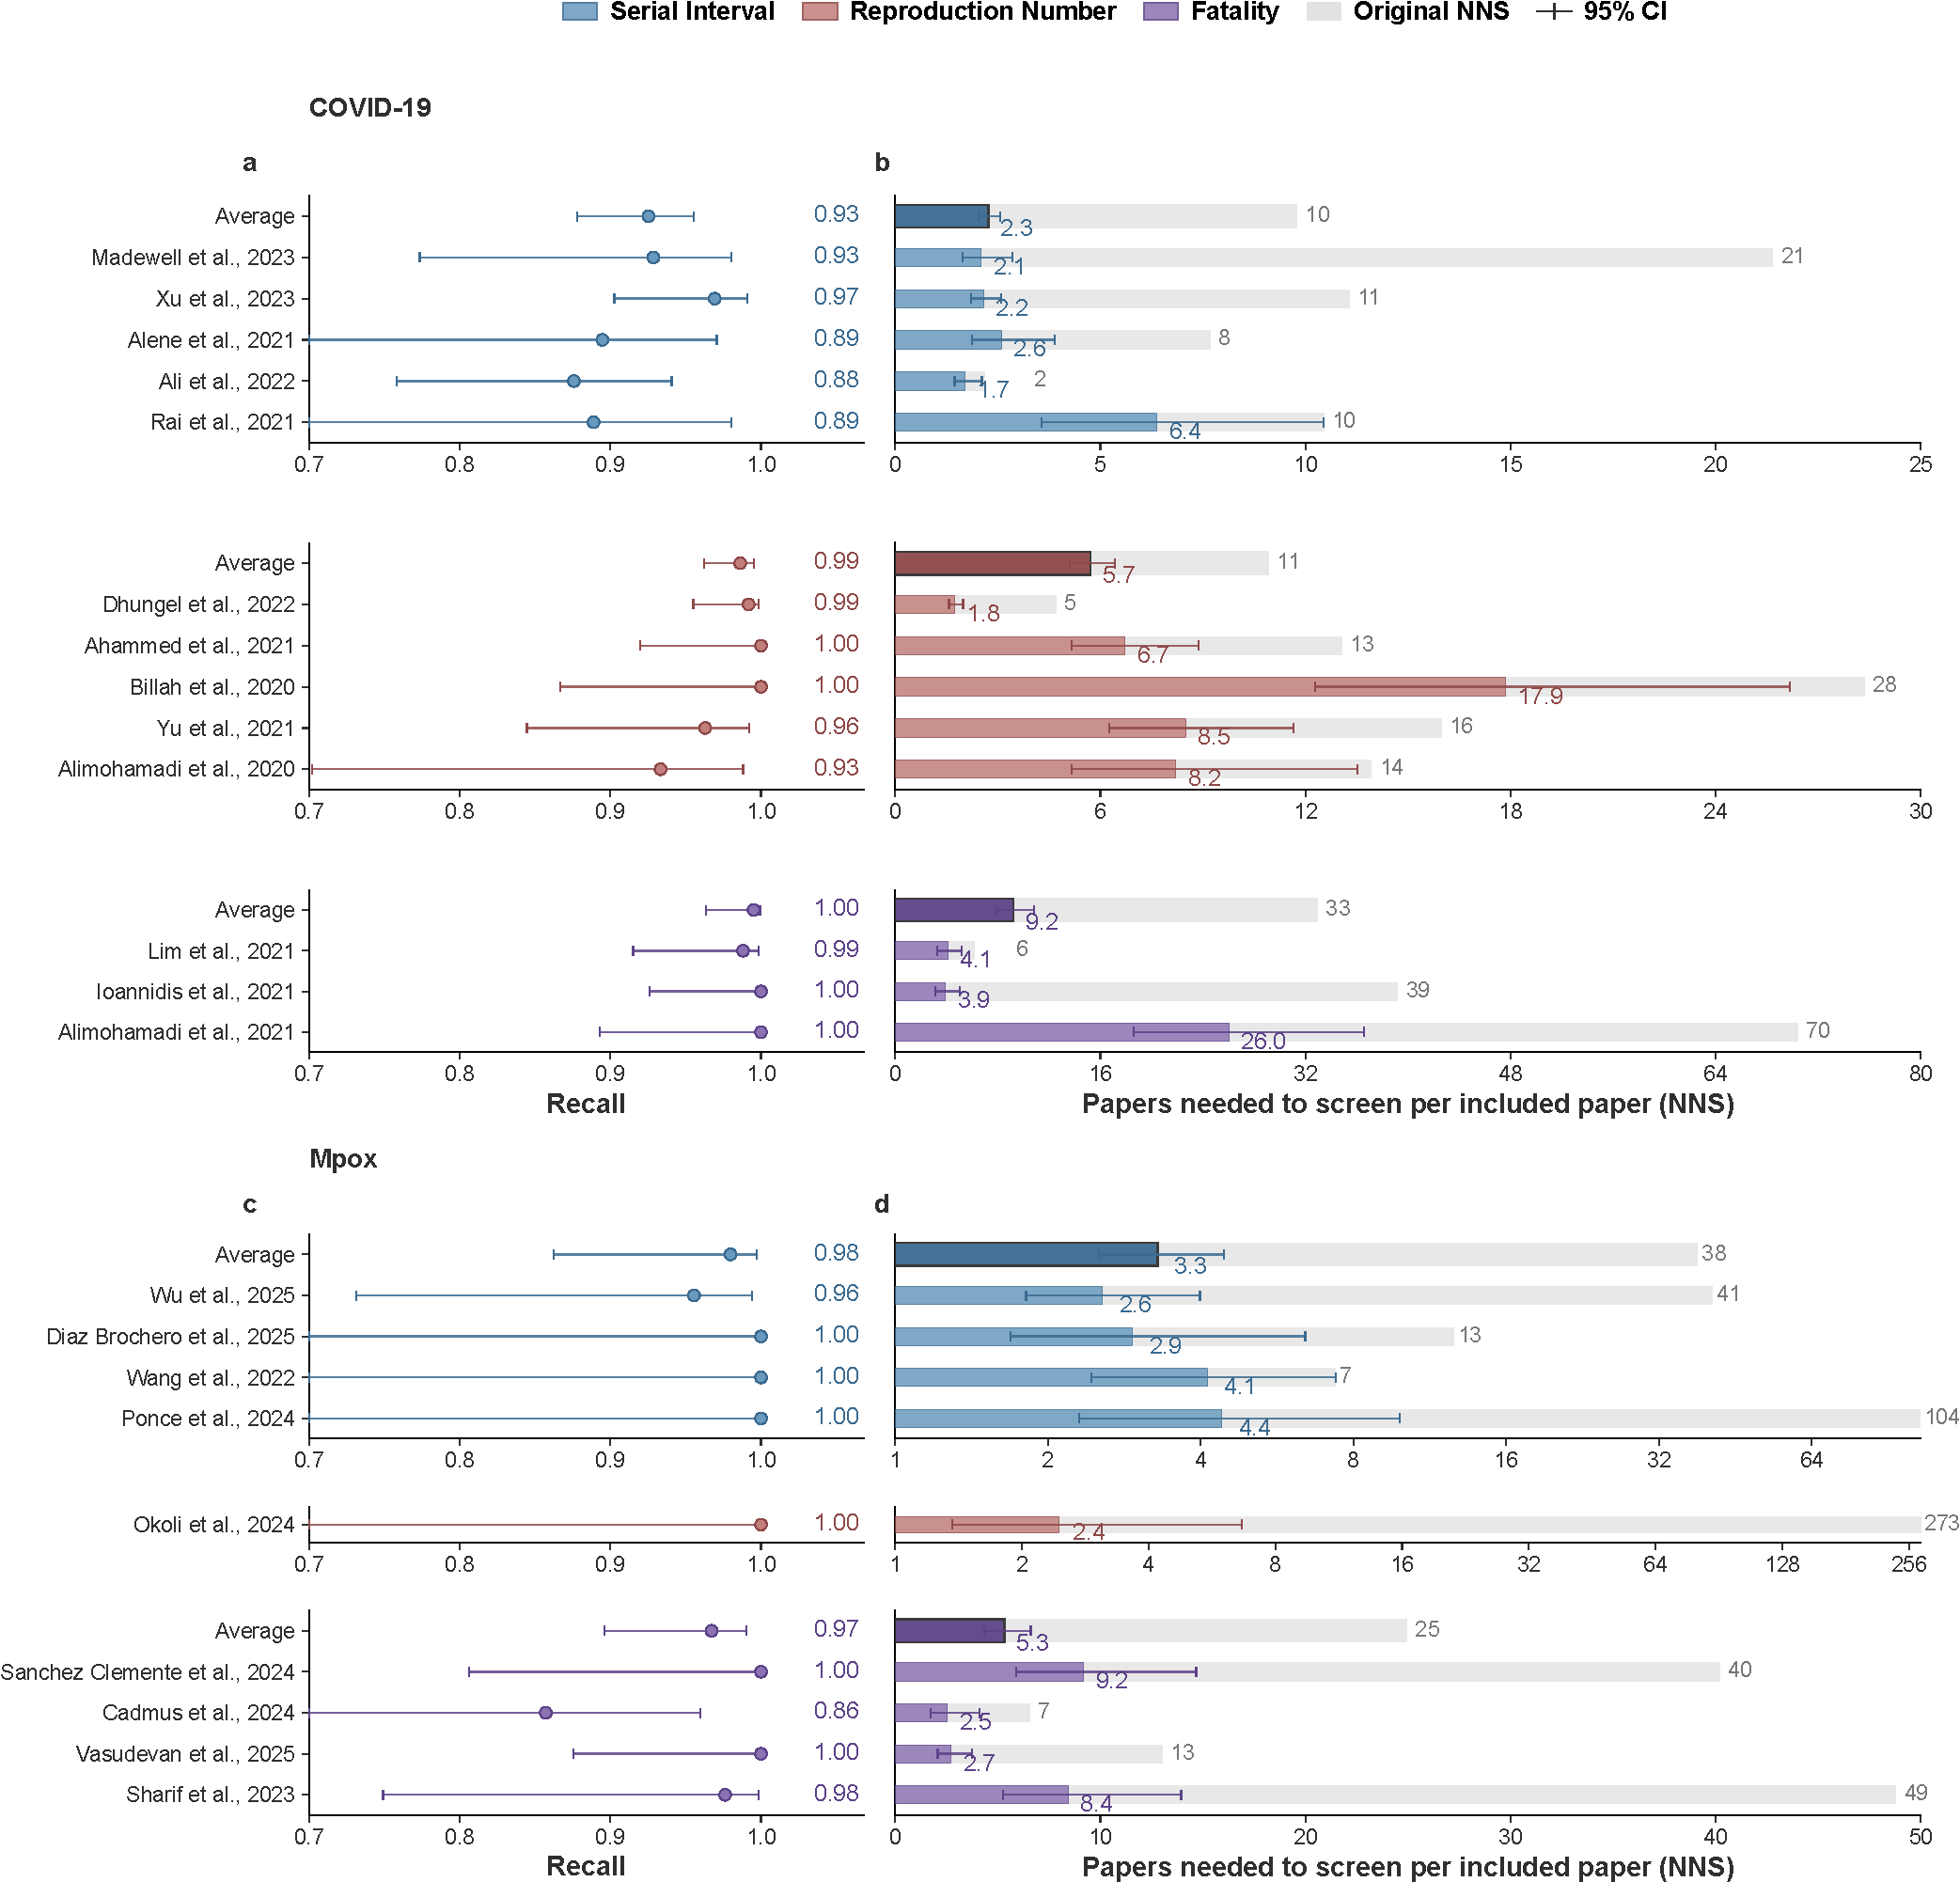
\includegraphics[width=\textwidth]{pdf/screening_recall_nns_overall.pdf}
  \caption{LLM-assisted screening recall and \nns{} (papers needed to screen per included paper) across COVID-19 and mpox benchmarks. a) and c) per-review recall grouped by parameter domain (colour-coded); filled circles are per-review recall; horizontal bars are Wilson 95\% CIs. b) and d) corresponding \nns{}; coloured bars = LLM-assisted, grey bars = original unassisted; whiskers are 95\% CIs.}
  \label{fig:screening-recall-nns}
\end{figure}

\subsection{Full-Text Parameter Coding and Extraction}

Full-text parameter coding and extraction recovered the source-review estimates with close agreement across the benchmark. This component-level analysis used the source-review included studies as fixed inputs, isolating the coding workflow from upstream screening errors, and tested whether localization and codebook-guided extraction could recover the evidence required to reproduce the review-level epidemiological estimates.

Across 22 source reviews, the LLM-coded estimates closely matched the source-review references (Figure~\ref{fig:coding-overall}). Agreement was strongest in reviews for which the target estimand and pooling rule were explicitly defined, as observed for the serial-interval and reproduction-number analyses. For COVID-19, LLM-coded serial-interval estimates differed from the source-review estimates by 0.02--0.09 days across all five reviews, and the reproduction-number estimates preserved the same review-level ordering as the original analyses. Fatality estimates were also recovered when the denominator was aligned with that of the source review, including invasive-mechanical-ventilation fatality, hospitalized fatality, and mpox clade- or population-specific CFR.

These observations were further supported by a supplementary comparison against the LEADS coding baseline (Appendix D). Because the target parameters are measured on different scales, agreement was interpreted primarily within parameter domains. The parameter-stratified MAE was 0.190 days for serial interval, 0.165 for reproduction number, and 0.416 pp for fatality; the mixed-unit overall MAE is reported as a descriptive summary in Appendix D. The codebook-guided workflow produced estimates closer to the source-review reference than LEADS in 21 of 22 source reviews, with the only exception being an incubation-period entry in which both methods remained close to the reference. Taken together, these results indicate that codebook-guided full-text coding can align LLM-coded estimates with source-review epidemiological estimates when the target parameter definition and synthesis rule are made explicit. Full per-review comparisons are reported in Figure~\ref{fig:supp-coding-leads} and Table~\ref{tab:coding-compare-leads-detail}.

\begin{figure}[!t]
  \centering
  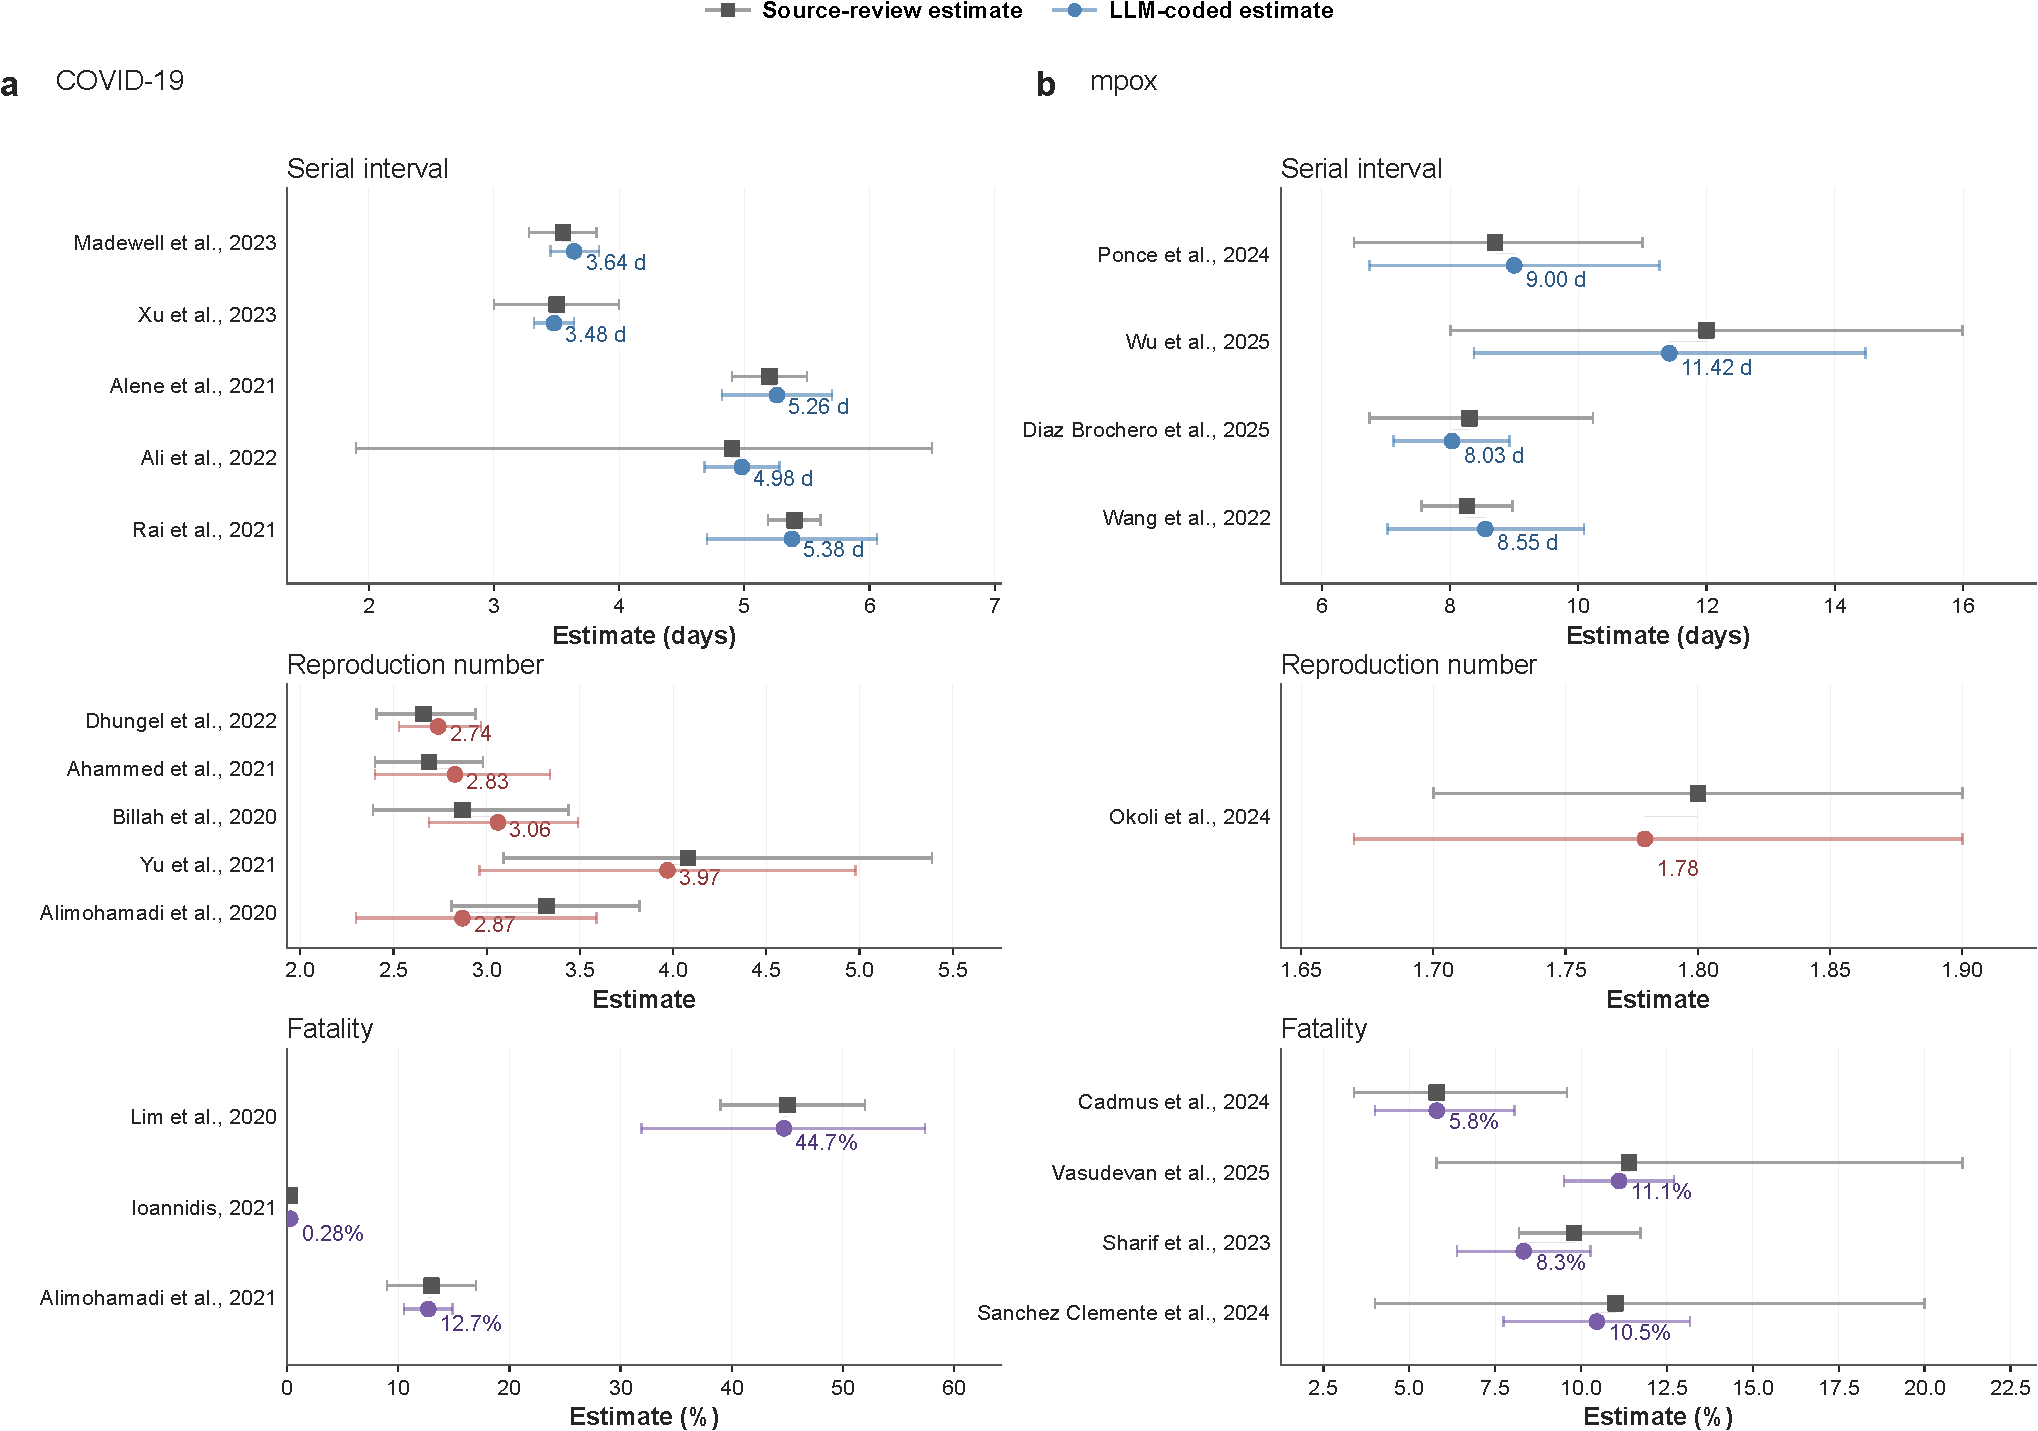
\includegraphics[width=\textwidth]{pdf/coding_estimates_overall_by_disease.pdf}
  \caption{Agreement between LLM-coded estimates and source-review estimates. Panels a and b show source-review and LLM-coded estimates for serial interval, reproduction number, and fatality in COVID-19 and mpox reviews. Points denote point estimates and horizontal bars denote 95\% confidence intervals. Grey squares indicate estimates reported in the source reviews; coloured circles indicate estimates derived from LLM-coded full-text evidence. Axes are scaled separately by disease and parameter.}
  \label{fig:coding-overall}
\end{figure}

\nocite{ref15,ref16,ref17,ref18,ref19,ref20,ref21,ref22,ref23,ref24,ref25,ref26,ref27}
% !TEX root = ../main.tex
\section{Discussion}

Systematic reviews provide the evidentiary foundation for characterizing infectious disease epidemics, yet their production remains constrained by labor-intensive screening and downstream evidence extraction. In this study, we developed \metagent{}, a structured LLM-assisted workflow for systematic reviews of infectious disease modeling parameters. Across 22 COVID-19 and mpox source-review screening tasks comprising 12,758 candidate records and 668 ground-truth included studies, \metagent{} achieved an overall recall of 0.960 while reducing the overall \nns{} from 19.10 to 5.25. Performance was consistent across three epidemiological parameter domains, with recall reaching 0.984 for reproduction number, 0.935 for serial interval, and 0.957 for fatality. These findings suggest that LLM-assisted screening can substantially reduce the number of records requiring human review while preserving the sensitivity required in systematic review workflows.

The screening module was designed to reflect the eligibility logic used by domain experts. Rather than relying on a single binary relevance judgment, \metagent{} generates criterion-specific scores and rationales for disease, population, location, empirical-evidence, and parameter criteria before assigning an overall Strong, Possible, or Unlikely triage label. This structure reflects the fact that eligibility in infectious disease parameter reviews is rarely determined by one criterion alone. For example, an article may focus on the correct disease but report no empirical estimate of the target parameter, or it may estimate a relevant parameter using non-human or purely theoretical data. The intermediate relevance categories provide a transparent representation of the screening decision, supporting human oversight and reducing the risk of premature exclusion.

The framework was intentionally optimized for recall rather than precision. In systematic review screening, false negatives are generally more consequential than false positives, because missed eligible studies may bias downstream evidence synthesis and parameter estimation. \metagent{} therefore treats both Strong and Possible articles as relevant for manual review. This conservative strategy explains the moderate overall precision but is appropriate for a first-pass screening tool whose purpose is not to replace expert judgment, but to prioritize records and reduce the screening burden. This is particularly critical in resource-constrained emergency settings, such as guiding evidence-based public health responses during sudden outbreaks. The reduction in \nns{} indicates that reviewers would need to screen fewer records for each eligible study retained, allowing reviewers to focus on a smaller and more enriched set of candidate studies.

Performance varied across parameter domains, reflecting differences in how epidemiological concepts are reported in the literature. Reproduction-number reviews achieved the highest recall (0.984), with fatality (0.957) and serial-interval (0.935) reviews also retaining high sensitivity. Although serial-interval recall was the lowest among the three domains, inspection of false negatives indicated that some eligible studies reported the target parameter only in full-text tables, appendices, or secondary analyses rather than in the abstract. This limitation is inherent to title-and-abstract screening and is not unique to LLM-based methods. Reproduction number tasks showed high recall but higher \nns{} than serial interval tasks, likely because broad mentions of transmissibility and epidemic growth make it more difficult to distinguish articles that estimate reproduction numbers from those that merely discuss them. These findings highlight that screening difficulty is partly determined by the semantic specificity of the target parameter. An analogous parameter-specific gradient was observed in full-text coding: fatality estimates required additional alignment of denominators and population strata before they could be compared with the source-review references, whereas serial-interval and reproduction-number estimates could be coded against more uniformly defined estimands. The screening- and coding-side challenges therefore share a common origin in the heterogeneity of how each target parameter is defined and reported, rather than in the discriminative capacity of the underlying model.

\metagent{} also addresses an important limitation of generic LLM applications in systematic review automation. Previous fully automated GPT-based approaches have shown limited ability to identify eligible articles in systematic reviews, underscoring the need for task-specific workflow design. In contrast, \metagent{} does not require domain-specific model retraining, but improves screening performance through structured prompting and explicit eligibility criteria applied to a uniform title-and-abstract input. This suggests that carefully designed LLM workflows, augmented with epidemiological domain knowledge and review-specific eligibility criteria, may provide practical gains even without model fine-tuning. Such a design may be especially valuable in rapidly evolving outbreak contexts, where timely evidence synthesis is needed but labeled training data may be limited.

Beyond screening, the full-text parameter coding and extraction experiment indicates that LLM-assisted workflows can support later stages of infectious disease meta-analysis when the included studies are fixed. The coding component did not attempt to replace full prospective review conduct; instead, it tested whether target-parameter evidence could be localized, coded, extracted, and aggregated to align with estimates reported by the source reviews. This distinction is important because parameter coding and extraction depend not only on identifying relevant papers, but also on aligning denominators, populations, estimands, and synthesis rules. The close agreement with source-review estimates therefore supports the feasibility of codebook-guided parameter coding and extraction, while preserving the need for expert adjudication when review definitions are ambiguous.

\metagent{} provides valuable assistance to medical experts and systematic reviewers by streamlining the literature mining process and offering superior temporal efficiency compared to purely manual efforts. However, the feasibility of AI integration remains constrained by several unresolved concerns, including algorithmic opacity, compromised reproducibility across temporally distinct queries, and limited capacity for context-dependent interpretation.\cite{ref28} Thus, while AI offers considerable potential as an adjunctive instrument for accelerating review workflows, a critical examination of its methodological boundaries and the enduring necessity of human oversight warrants further investigation.\cite{ref29,ref30}

Despite these strengths, several limitations should be considered. First, the ground truth was derived from the inclusion lists of published systematic reviews rather than from a newly adjudicated gold standard. Published reviews may contain retrieval omissions, apply eligibility criteria that are incompletely reported, or include studies identified through databases and supplementary searches not reproduced in our benchmark. As a result, recall and precision estimates should be interpreted as performance against review-derived ground truth, not as definitive measures against an exhaustive corpus of all eligible studies. Second, our benchmark was constructed primarily from PubMed, whereas the original systematic reviews often searched multiple bibliographic databases. This structural asymmetry may limit the generalizability of the reported performance to complete real-world systematic review workflows involving Embase, Web of Science, Scopus, preprint servers, and manual citation tracking. Third, the full-text screening comparison and parameter coding analysis were evaluated as controlled experiments rather than as a fully prospective end-to-end review. Articles labeled Strong or Possible still require expert review, and final inclusion decisions remain the responsibility of human reviewers. Fourth, the method depends on the information available in titles, abstracts, accessible full texts, and parsed tables. Studies that report relevant parameters only in supplementary materials, images, or poorly parsed tables may still be missed or incompletely coded. The focused full-text screening comparison suggests that access to full-text evidence can improve both sensitivity and specificity when relevant evidence is absent from the abstract, but this benefit was conditional on successful full-text retrieval and parsing. In practice, many records lack informative abstracts, are not available through PMC Open Access or other accessible full-text sources, or contain the relevant parameter only in tables, appendices, or sections that are difficult to localize automatically. These constraints point to an infrastructure-level limitation of current evidence synthesis workflows: more open, structured, and machine-readable repositories of biomedical full text, tables, supplementary materials, and review-level extraction targets would likely improve both LLM-assisted screening and downstream parameter coding. Incorporating broader full-text retrieval and multimodal table understanding may reduce this source of error, but would introduce additional challenges related to access, document parsing, and computational cost.

More broadly, integrating LLMs into evidence synthesis raises methodological and operational concerns. LLM outputs may vary across model versions, prompts, and time, affecting reproducibility. The internal reasoning process of proprietary models may not be fully transparent, and model behavior may shift as systems are updated. These issues are particularly important for systematic reviews, where reproducibility and auditability are central methodological principles. The structured decision design of \metagent{} improves interpretability at the decision level, but does not eliminate the need for careful documentation, version control, prompt archiving, and human verification.

Future work should evaluate \metagent{} prospectively in live systematic review projects and across a wider range of pathogens, study designs, and epidemiological parameters. Multi-database benchmarks would better reflect real-world search workflows, while prospective validation could assess how the system performs when screening newly published literature not available during model pretraining. Further development should also explore integration with full-text screening, citation chasing, uncertainty calibration, and active-learning prioritization. Combining LLM-based semantic assessment with conventional information retrieval methods may further improve both sensitivity and efficiency. In parallel, the coding and extraction component warrants dedicated extension. Promising directions include multimodal table and figure understanding for parameter values that are not represented in running text, automatic harmonization of denominators and estimands across reviews, transferable codebooks that generalize to new pathogens or parameter families, and uncertainty-aware aggregation that explicitly propagates extraction confidence into downstream meta-analytic estimates. Joint optimization of retrieval and parameter-aware coding within a single human-in-the-loop framework may further narrow the gap between LLM-assisted output and review-ready evidence synthesis.

In summary, \metagent{} demonstrates that structured LLM-assisted workflows can support systematic reviews of infectious disease modeling parameters. The framework preserves high screening recall, lowers \nns{}, and assists full-text parameter coding and extraction as a modular component of evidence synthesis. These results support the use of structured, human-in-the-loop LLM systems as complementary infrastructure for systematic reviews, particularly in public health settings where timely and reliable parameter evidence is essential.

\clearpage
\nocite{ref31,ref32,ref33,ref34,ref35,ref36,ref37,ref38,ref39}
\bibliographystyle{unsrtnat-nodoi}
\bibliography{references}
% !TEX root = ../main.tex
\clearpage
\appendix
\phantomsection
\addcontentsline{toc}{section}{Appendix}
\section*{Appendix}
\setcounter{figure}{0}
\renewcommand{\thefigure}{S\arabic{figure}}
\setcounter{table}{0}
\renewcommand{\thetable}{S\arabic{table}}

\phantomsection
\addcontentsline{toc}{subsection}{Appendix A. Metric Definitions}
\subsection*{Appendix A. Metric Definitions}

For each model evaluated on the screening benchmark, the following metrics are reported.
TP = true positives (included papers correctly retrieved);
FP = false positives (excluded papers incorrectly retrieved);
FN = false negatives (included papers missed);
TN = true negatives (excluded papers correctly excluded).
\[
\text{Recall} = \frac{\text{TP}}{\text{TP}+\text{FN}},
\quad
\text{Precision} = \frac{\text{TP}}{\text{TP}+\text{FP}},
\quad
F_1 = \frac{2 \times \text{Precision} \times \text{Recall}}{\text{Precision}+\text{Recall}}.
\]
\[
\text{NNS} = \frac{\text{TP}+\text{FP}}{\text{TP}},
\quad
\text{WR} = 1 - \frac{\text{TP}+\text{FP}}{\text{TP}+\text{FP}+\text{FN}+\text{TN}}.
\]
\[
\text{Excluded GT rate} = \frac{\text{FN}}{\text{FN}+\text{TN}}.
\]

\clearpage

\phantomsection
\addcontentsline{toc}{subsection}{Appendix B. Screening Model Comparison}
\subsection*{Appendix B. Screening Model Comparison}

Supplementary Figure~\ref{fig:model-compare} visualizes recall and papers needed to screen across candidate models and baselines. Table~\ref{tab:model-summary} reports the corresponding aggregate counts and metrics on the unified benchmark. The LEADS screening baseline follows the official LEADS title-and-abstract screening use case, using a disease- and parameter-specific prompt and returning a binary include/exclude decision. Prompt templates for the proposed workflow are provided in Appendix F.

\begin{figure}[H]
  \centering
  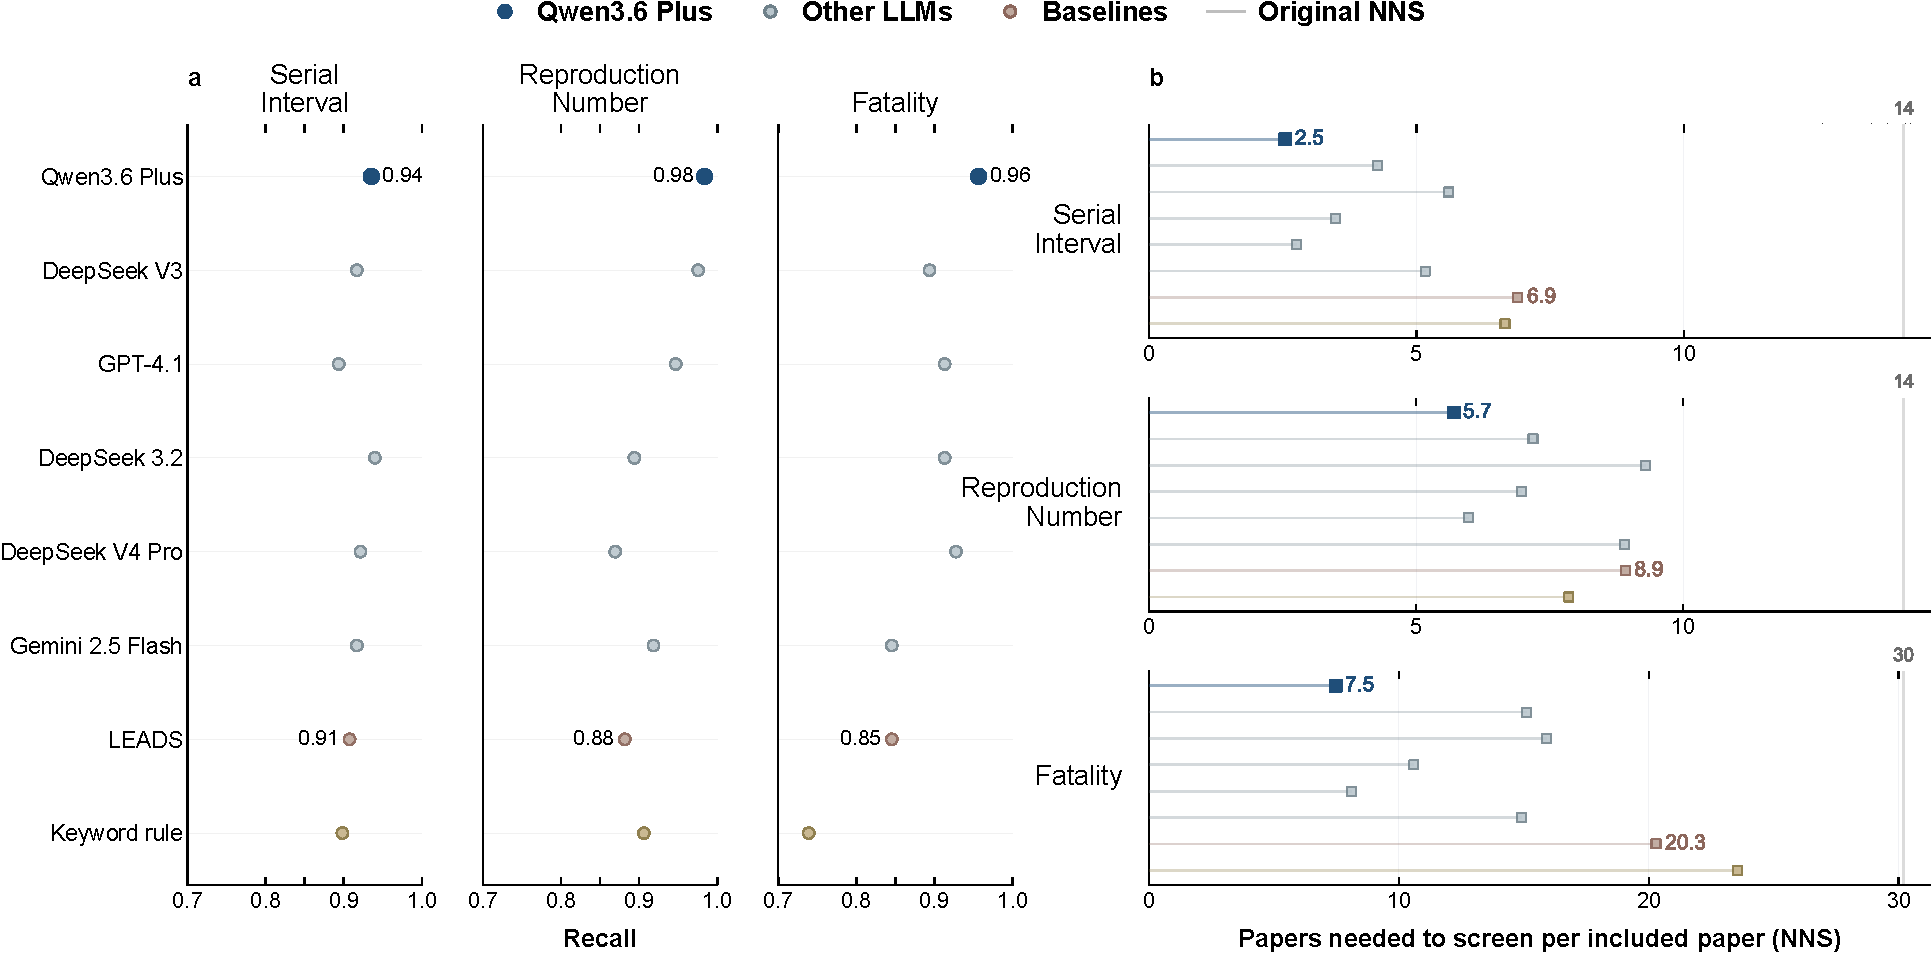
\includegraphics[width=\textwidth]{pdf/model_recall_nns_benchmark.pdf}
  \caption{Model-assisted screening performance across epidemiological parameters. a) Recall across three parameter domains, shown as dot plots to emphasize small differences among high-recall models. b) Papers needed to screen per included paper (\nns{}), where lower values indicate fewer papers screened per included paper; numbers above each panel indicate the original unassisted NNS.}
  \label{fig:model-compare}
\end{figure}

\papertable{model_summary.tex}

\clearpage

\phantomsection
\addcontentsline{toc}{subsection}{Appendix C. Second-Stage Full-Text Rescreening Analysis}
\subsection*{Appendix C. Second-Stage Full-Text Rescreening Analysis}

Tables~\ref{tab:fulltext-tier2-p13} and \ref{tab:p13-remaining-fp-audit} summarize a controlled comparison between title-and-abstract screening and full-text screening for the COVID-19 serial-interval review by Ali et al. 2022. The Ali et al. review was selected because it offered an appropriately sized raw pool and one of the largest sets of ground-truth included studies among the serial-interval tasks, providing sufficient signal to compare title-and-abstract and full-text inputs at the screening stage. Using the same five-criterion screening prompt and the same Strong, Possible, or Unlikely triage rule, screening was repeated with parsed full-text passages substituted for the title and abstract, while all other workflow components were held constant. Here, Stage II denotes this experimental full-text screening condition applied to records stratified by the Stage I title-and-abstract labels, not a required second step in the main screening pipeline.

\papertable{fulltext_tier2_p13_ablation.tex}

\papertable{fulltext_tier2_p13_remaining_fp_audit.tex}

\clearpage

\phantomsection
\addcontentsline{toc}{subsection}{Appendix D. Full-Text Parameter Coding and Extraction Comparison}
\subsection*{Appendix D. Full-Text Parameter Coding and Extraction Comparison}

Supplementary Figure~\ref{fig:supp-coding-leads} and Tables~\ref{tab:coding-leads-summary}--\ref{tab:coding-compare-leads-detail} provide the full per-source-review coding comparison between MetaAgent and LEADS. The detail table lists the source-review reference estimate used as the comparison target for each source review.

\begin{figure}[H]
  \centering
  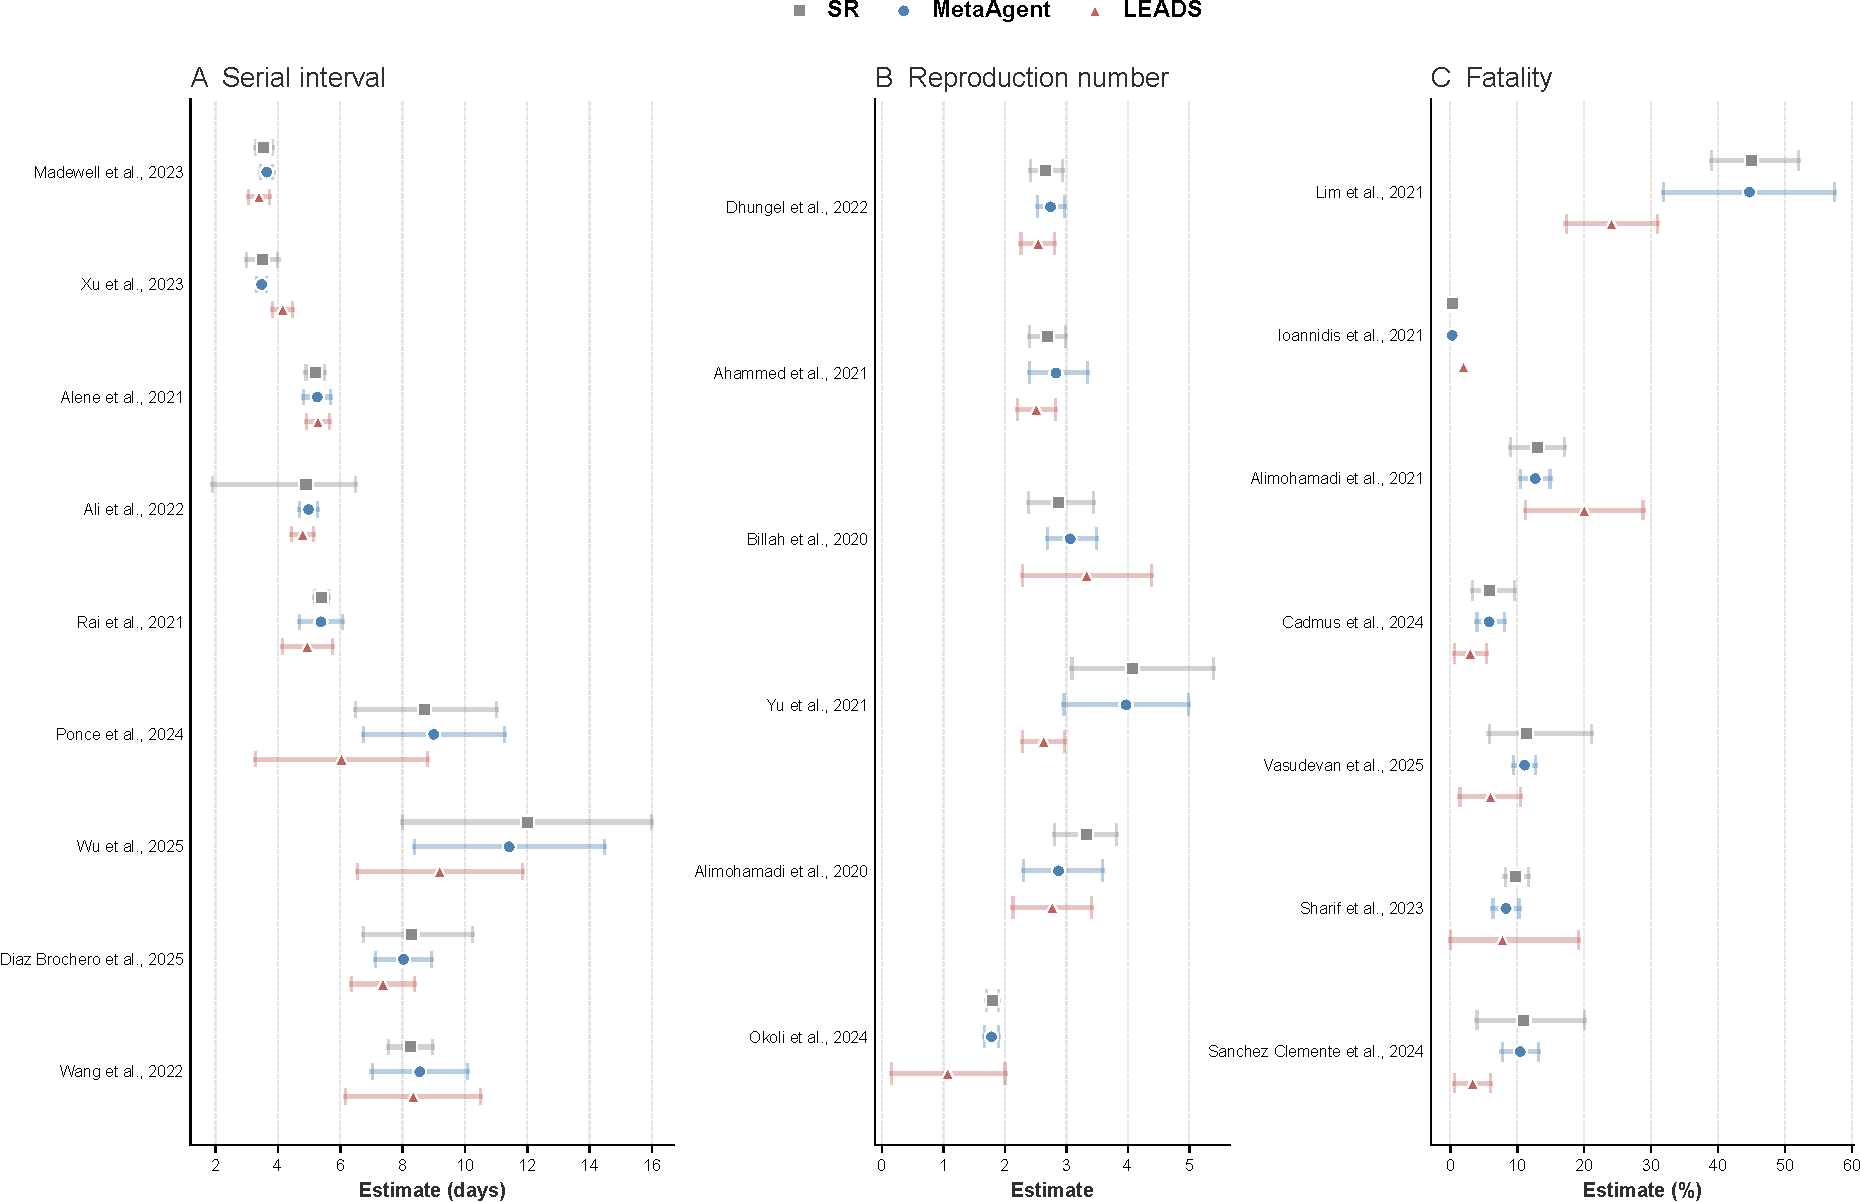
\includegraphics[width=\textwidth]{pdf/coding_compare_leads_official_final.pdf}
  \caption{Supplementary coding comparison of source-review (SR), MetaAgent, and LEADS estimates across serial interval, reproduction number, and fatality.}
  \label{fig:supp-coding-leads}
\end{figure}

\papertable{coding_compare_leads_summary.tex}

\papertable{coding_compare_leads_detail.tex}

\clearpage

\phantomsection
\addcontentsline{toc}{subsection}{Appendix E. Benchmark Source-Review Inventory}
\subsection*{Appendix E. Benchmark Source-Review Inventory}

Table~\ref{tab:source-reviews} lists the source reviews used to construct the frozen screening and coding benchmark.

\papertable{source_reviews.tex}

\clearpage

\phantomsection
\addcontentsline{toc}{subsection}{Appendix F. Prompt Specifications}
\subsection*{Appendix F. Prompt Specifications}

The prompt templates below summarize the stable runtime structure used in the screening and full-text coding workflows. Project-specific disease names, parameter names, source-review questions, screening-profile guidance, codebook fields, and JSON schema constraints were filled programmatically at run time. Long parameter-specific examples and implementation-level formatting constraints are abbreviated for readability.

\begin{prompttemplate}{Template F1. Title-and-abstract screening}
\textbf{System role and task.} You are assisting with title-and-abstract screening for an epidemiological systematic review. Score the study on five relevance dimensions and classify it into one of three tiers using holistic judgment.

\textbf{Review context.} Use the following source-review fields:
\begin{promptitems}
  \item Research question: \promptvar{research\_question}.
  \item Disease focus and exclusions: \promptvar{disease\_focus}; \promptvar{disease\_exclude}.
  \item Target parameter and exclusions: \promptvar{parameter\_focus}; \promptvar{parameter\_exclude}.
\end{promptitems}

\textbf{Available evidence.} Use the title, abstract, publication year, record/create date, keywords, publication types, and MeSH terms. If the abstract is missing or sparse, avoid over-certainty and retain only records with concrete parameter or outcome cues.

\textbf{Assessment dimensions.} Score each dimension from 0 to 4 with a concise evidence-based rationale:
\begin{promptitems}
  \item Disease relevance: whether the paper investigates the target disease.
  \item Population relevance: whether the paper concerns humans or human-derived data.
  \item Location relevance: whether the study reports data from a real-world geographic setting relevant to the source review.
  \item Original empirical evidence: whether the paper reports original empirical data or primary analysis rather than only review, commentary, or theoretical content.
  \item Target-parameter relevance: whether the paper reports, estimates, or plausibly contains the target epidemiological parameter.
\end{promptitems}

\textbf{Parameter-specific guidance.} Apply the profile-specific guidance for the current disease and parameter domain. This guidance defined accepted synonyms, related quantities to distinguish, and common exclusion patterns; detailed edge-case examples are abbreviated here.

\textbf{Triage output.} Assign exactly one tier:
\begin{promptitems}
  \item \textbf{S}: strong candidate; clear evidence for the target disease, original empirical evidence, and target parameter.
  \item \textbf{P}: possible candidate; plausible but incomplete or ambiguous evidence requiring human review or full-text verification.
  \item \textbf{U}: unlikely candidate; no plausible match to one or more core eligibility criteria.
\end{promptitems}

\textbf{Response format.} Return JSON only. Include the five dimension scores and rationales, an optional overall score and confidence, the final S/P/U tier, and a short overall justification. The runtime prompt additionally supplied the JSON schema constraint.
\end{prompttemplate}

\begin{prompttemplate}{Template F2. Full-text evidence localization}
\textbf{System role and task.} You are an epidemiology research assistant creating a structured index from the full text of a primary study. Use only evidence from the provided text; do not guess or infer unsupported values. This is a high-recall indexing stage, not final extraction.

\textbf{Input.} Use \promptvar{title}, \promptvar{abstract}, parsed full text, recoverable tables and captions, and the parameter-domain codebook.

\textbf{Indexing targets.} Identify document sections, tables, figure captions, and paragraphs that may contain evidence for the target parameter, uncertainty interval, sample size, numerator or denominator, population, geography, study period, estimation method, or review-specific synthesis rule. Domain-specific prompts emphasized serial-interval, reproduction-number, or fatality evidence as appropriate.

\textbf{Response format.} Return JSON only. Summarize document structure, relevant tables, study metadata, parameter mentions, analysis summaries when applicable, and field-level evidence locations. Use null or empty arrays when evidence is not found.
\end{prompttemplate}

\begin{prompttemplate}{Template F3. Full-text parameter coding and extraction}
\textbf{System role and task.} You are an epidemiology meta-analyst extracting codebook-defined records from a full-text article. Use only evidence from the provided text and the Stage-A index; do not guess or compute values unless explicitly instructed by the codebook.

\textbf{Input.} Use \promptvar{title}, \promptvar{abstract}, parsed full text, recoverable table summaries, the Stage-A evidence index, and the parameter-specific codebook.

\textbf{Extraction rules.} Extract the study-level record or records needed for the source-review parameter analysis. Follow field definitions strictly; preserve reported point estimates, uncertainty intervals, units, denominators, populations, study periods, and evidence locations. Prefer the headline or overall estimate unless the source-review codebook specifies a subgroup or denominator. Parameter-domain rules distinguished serial interval from related timing quantities, $R_0$ from $R_t$ and assumed model inputs, and CFR from IFR, hospitalized fatality, ICU fatality, or denominator-specific fatality estimates.

\textbf{Response format.} Return a JSON array only. Each record includes the codebook-defined fields, including parameter type, point estimate, uncertainty interval when reported, population or subgroup, study period, geography, numerator or denominator where applicable, evidence location, and notes. Use null for missing numeric fields and ``NR'' for required text fields that are not reported. The runtime prompt also supplied codebook-specific field descriptions and an example JSON output.
\end{prompttemplate}


\clearpage
\section*{Acknowledgements}
To be completed.

% \section*{Author Contributions}
% To be completed.

% \section*{Competing Interests}
% The authors declare no competing interests.

\section*{Data Availability}
Coming soon.

\section*{Code Availability}
Coming soon.

\end{document}
